\documentclass[11pt,a4paper]{article}
\usepackage[utf8]{inputenc}
\usepackage[T1]{fontenc}
\usepackage[brazil]{babel}
\usepackage{lmodern}
\usepackage[margin=2.5cm]{geometry}
\usepackage{amsmath,amssymb}
\usepackage{graphicx}
\usepackage{booktabs}
\usepackage{float}
\usepackage{caption}
\usepackage{xcolor}
\usepackage{listings}
\usepackage[hidelinks]{hyperref}
\graphicspath{{../figuras/}}

\lstset{language=R, basicstyle=\ttfamily\scriptsize, breaklines=true, frame=single,
  commentstyle=\color{gray}, keywordstyle=\color{blue!60!black}, stringstyle=\color{green!40!black},
  columns=fullflexible, showstringspaces=false}
\makeatletter\newcommand{\linhas}[1]{\@@input #1 }\makeatother
\newcommand{\E}{\mathrm{E}}
\newcommand{\Var}{\mathrm{Var}}

\begin{document}

\begin{titlepage}
\centering
{\large Universidade de São Paulo\\ Instituto de Ciências Matemáticas e de Computação}\\[1.5cm]
{\large SME0809 -- Inferência Bayesiana}\\
{\large Prof. Adriano K. Suzuki}\\[2.5cm]
{\LARGE\bfseries Inferência clássica e bayesiana para a\\[0.2cm] distribuição moment exponential discreta}\\[0.5cm]
{\large com aplicação a mortes diárias por COVID-19}\\[2.5cm]
\begin{tabular}{ll}
Antônio Carlos Cavalcante Gonçalves & 16854872\\
Caio Corrêa Chaves & 15444406\\
Caique Figueiredo Freitas & 11836121\\
Francisco Chiarello Ferreira & 16228894\\
João Vitor Costa Morais Lemes & 16877300\\
Paulo Eduardo De Vincenzi & 12743130\\
Pedro Paulo Silva Santos & 16993206
\end{tabular}
\vfill
São Carlos\\ Novembro de 2026
\end{titlepage}

\tableofcontents
\newpage

% =====================================================================
\section{Introdução}

Dados de contagem com grande dispersão, como o número diário de mortes em uma epidemia, raramente são bem descritos pela Poisson, cuja variância é igual à média. Uma estratégia comum para construir modelos discretos mais flexíveis é \emph{discretizar} uma distribuição contínua: se $Y$ é contínua e positiva, $X=\lfloor Y\rfloor$ é uma contagem cuja função de probabilidade herda a forma de $Y$. Esse método da função de sobrevivência gerou, por exemplo, a Weibull discreta \cite{nakagawa1975} e a Rayleigh discreta \cite{roy2004}.

Afify et al. \cite{afify2022} aplicaram esse método à distribuição \emph{moment exponential} (MEx) de \cite{dara2012}, isto é, à exponencial ponderada pelo comprimento, cuja densidade é $f(y)=y\,\beta^{-2}e^{-y/\beta}$. O resultado é a \emph{moment exponential discreta} (DMEx), com um único parâmetro $\beta>0$. Os autores estudaram suas propriedades, compararam sete estimadores \emph{clássicos} (máxima verossimilhança, mínimos quadrados, Cramér--von Mises, Anderson--Darling etc.) por simulação e ajustaram o modelo às mortes diárias por COVID-19 na China e na Europa no início de 2020. O artigo não tem inferência bayesiana.

Este trabalho refaz o estudo com as ferramentas atuais e acrescenta a parte bayesiana:
\begin{itemize}
\item deduzimos as propriedades, a verossimilhança e a função escore do modelo;
\item propomos duas prioris para $\beta$: uma Gama vaga e a priori $\pi(\beta)\propto1/\beta$, e mostramos quando a posteriori desta última é própria;
\item comparamos por simulação o estimador de máxima verossimilhança (EMV) e a média a posteriori (viés, EQM, cobertura), usando as \emph{mesmas} amostras para os dois;
\item refazemos a aplicação aos dados de COVID-19 com os dois paradigmas, incluindo concorrentes (Poisson, geométrica, binomial negativa e Weibull discreta) e critérios bayesianos (DIC, WAIC e LPML).
\end{itemize}

A priori $1/\beta$ tem uma motivação clássica. \cite{lindley1958} mostrou que a distribuição fiducial de Fisher coincide com uma posteriori de Bayes se, e somente se, existe uma transformação que torna o parâmetro de locação (condição (A)). Nesse caso, a priori correspondente é uniforme no parâmetro de locação. Na Gama contínua, $\beta$ é parâmetro de escala, logo $\tau=\log\beta$ é de locação e a priori é $\pi(\beta)\propto1/\beta$. Após a discretização, a condição (A) deixa de valer exatamente, e é natural perguntar quanto essa priori ainda se comporta como ``não informativa''.

% =====================================================================
\section{Modelo}

\subsection{Construção}

Seja $Y\sim\text{Gama}(2,\beta)$, com forma 2 e escala $\beta$, isto é, $f_Y(y)=y\beta^{-2}e^{-y/\beta}$, $y>0$. Essa é a MEx: a densidade da exponencial de média $\beta$ ponderada por $y$. Integrando por partes, a função de sobrevivência é
\begin{equation}
S(y)=P(Y>y)=\int_y^\infty \frac{t}{\beta^2}e^{-t/\beta}\,dt=\Big(1+\frac{y}{\beta}\Big)e^{-y/\beta}.
\end{equation}
Definimos $X=\lfloor Y\rfloor$. Como $\{X=x\}=\{x\le Y<x+1\}$,
\begin{equation}
p(x;\beta)=P(X=x)=S(x)-S(x+1),\qquad x=0,1,2,\dots
\end{equation}

\subsection{Propriedades}

\paragraph{Função de probabilidade.} Com $u=1/\beta$ e $q=e^{-u}$,
\begin{align}
p(x;\beta)&=e^{-xu}\big[(1+xu)-(1+(x+1)u)q\big]
=e^{-xu}\Big[\underbrace{1-(1+u)q}_{P(\text{Gama}(2,1)\le u)}+x\,u\,(1-q)\Big]\equiv e^{-xu}A(x;\beta). \label{eq:fmp}
\end{align}
A segunda forma evita subtrair números próximos e é a usada no código. Como $A>0$, $p(x;\beta)>0$ para todo $x$. A soma é telescópica: $\sum_{x\ge0}p(x)=S(0)-\lim_{x\to\infty}S(x)=1$.

\paragraph{Função de distribuição e sobrevivência.}
\begin{equation}
F(x)=P(X\le x)=1-S(x+1)=1-\Big(1+\frac{x+1}{\beta}\Big)e^{-(x+1)/\beta},\qquad P(X\ge x)=S(x).
\end{equation}
A taxa de falha discreta é $h(x)=p(x)/S(x)=1-\dfrac{1+(x+1)u}{1+xu}\,q$, crescente em $x$ e com limite $1-q$. Ou seja, a DMEx tem taxa de falha crescente, como a Gama de forma 2.

\paragraph{Momentos.} Para $X$ inteiro não negativo, $\E(X)=\sum_{k\ge1}P(X\ge k)=\sum_{k\ge1}S(k)$ e $\E(X^2)=\sum_{k\ge1}(2k-1)S(k)$. Usando $S(k)=q^k(1+ku)$ e as séries $\sum_{k\ge1}kq^k=q/(1-q)^2$ e $\sum_{k\ge1}k^2q^k=q(1+q)/(1-q)^3$:
\begin{align}
\E(X)&=\frac{q}{1-q}+\frac{u\,q}{(1-q)^2},\\
\E(X^2)&=2\left[\frac{q}{(1-q)^2}+\frac{u\,q(1+q)}{(1-q)^3}\right]-\E(X),\qquad \Var(X)=\E(X^2)-\E(X)^2.
\end{align}
Para $\beta$ grande, $\E(X)\approx2\beta-\tfrac12$ e $\Var(X)\approx2\beta^2+\tfrac1{12}$, pois $X\approx Y-U$ com $U$ aproximadamente uniforme em $(0,1)$. Daí seguem duas consequências:
\begin{itemize}
\item o índice de dispersão $\Var(X)/\E(X)\approx\beta$ indica sobredispersão para $\beta>1$;
\item o coeficiente de variação é praticamente fixo, $\text{CV}\approx1/\sqrt2\approx0{,}71$, como na Gama de forma 2.
\end{itemize}
Essa rigidez do CV vai ser importante na aplicação. As expressões foram conferidas numericamente contra $10^6$ simulações (script \texttt{00\_checagens.R}). A Figura~\ref{fig:fmp} mostra a fmp e a fda para os valores de $\beta$ usados na simulação.

\begin{figure}[H]\centering
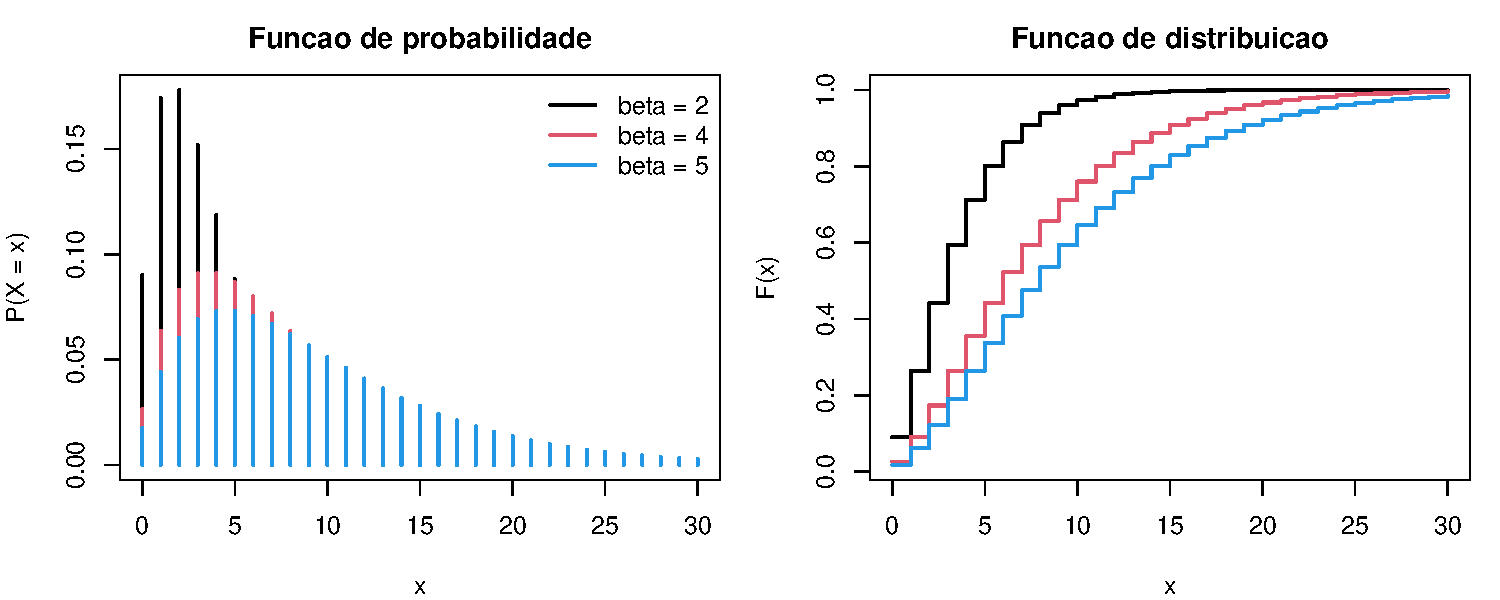
\includegraphics[width=\linewidth]{fmp_dmex.pdf}
\caption{Função de probabilidade e função de distribuição da DMEx para $\beta\in\{2,4,5\}$.}\label{fig:fmp}
\end{figure}

\paragraph{Geração.} Como $Y\sim\text{Gama}(2,\beta)$ é a soma de duas exponenciais independentes de média $\beta$, se $U_1,U_2\sim U(0,1)$ são independentes, então
\[
X=\big\lfloor -\beta\log(U_1U_2)\big\rfloor\sim\text{DMEx}(\beta).
\]
No R usamos o equivalente \texttt{floor(rgamma(n, shape = 2, scale = beta))}.

% =====================================================================
\section{Metodologias inferenciais}

Seja $\mathbf x=(x_1,\dots,x_n)$ uma amostra aleatória da DMEx($\beta$).

\subsection{Abordagem clássica}

\paragraph{Log-verossimilhança.} Por \eqref{eq:fmp},
\begin{equation}
\ell(\beta)=\sum_{i=1}^n\log p(x_i;\beta)=-\frac1\beta\sum_{i=1}^nx_i+\sum_{i=1}^n\log A(x_i;\beta).
\end{equation}

\paragraph{Função escore.} Derivando a sobrevivência em $\beta$:
\[
\frac{\partial S(y)}{\partial\beta}=-\frac{y}{\beta^2}e^{-y/\beta}+\Big(1+\frac y\beta\Big)\frac{y}{\beta^2}e^{-y/\beta}=\frac{y^2}{\beta^3}e^{-y/\beta}.
\]
Logo $\partial p(x;\beta)/\partial\beta=\beta^{-3}\big[x^2e^{-xu}-(x+1)^2e^{-(x+1)u}\big]$. Dividindo por $p(x;\beta)=e^{-xu}A(x;\beta)$, obtemos
\begin{equation}
U(\beta)=\frac{\partial\ell}{\partial\beta}=\frac{1}{\beta^3}\sum_{i=1}^n\frac{x_i^2-(x_i+1)^2e^{-1/\beta}}{A(x_i;\beta)}.
\end{equation}
A equação $U(\hat\beta)=0$ não tem solução fechada. Maximizamos $\ell$ em $\eta=\log\beta$, cujo escore é $U_\eta=\beta\,U(\beta)$, pelo método BFGS com esse gradiente analítico. O escore analítico foi conferido contra a derivada numérica (script \texttt{00\_checagens.R}).

\paragraph{Erro padrão e intervalo.} Com $J(\hat\eta)=-\partial^2\ell/\partial\eta^2|_{\hat\eta}$ (informação observada, obtida da hessiana numérica):
\begin{itemize}
\item $\widehat{\text{EP}}(\hat\eta)=J(\hat\eta)^{-1/2}$;
\item pelo método delta, $\widehat{\text{EP}}(\hat\beta)=\hat\beta\,J(\hat\eta)^{-1/2}$;
\item o IC de 95\% é $\exp\{\hat\eta\pm1{,}96\,J(\hat\eta)^{-1/2}\}$, construído na escala $\eta$ e por isso sempre positivo.
\end{itemize}
Para comparar modelos usamos $\text{AIC}=-2\ell(\hat\theta)+2k$ e $\text{BIC}=-2\ell(\hat\theta)+k\log n$.

\subsection{Abordagem bayesiana}

\paragraph{Priori 1 (Gama vaga).} $\beta\sim\text{Gama}(a=0{,}1;\,b=0{,}01)$, com forma $a$ e taxa $b$: média 10 e variância 1000. A posteriori é
\begin{equation}
\pi_1(\beta\mid\mathbf x)\propto\beta^{a-1}e^{-b\beta}\exp\Big(-\frac{\sum_ix_i}{\beta}\Big)\prod_{i=1}^nA(x_i;\beta).
\end{equation}

\paragraph{Priori 2 (escala, Lindley/Jeffreys).} $\pi(\beta)\propto1/\beta$, isto é, uniforme em $\eta=\log\beta$:
\begin{equation}
\pi_2(\beta\mid\mathbf x)\propto\beta^{-1}\exp\Big(-\frac{\sum_ix_i}{\beta}\Big)\prod_{i=1}^nA(x_i;\beta).
\end{equation}
Nenhuma das duas tem forma conhecida, por isso usamos MCMC.

\paragraph{Propriedade de $\pi_2$.} A priori $1/\beta$ é imprópria nas duas pontas, então é preciso verificar a integrabilidade de $\beta^{-1}L(\beta)$ em cada uma.
\begin{itemize}
\item Quando $\beta\to\infty$ ($u\to0$), $1-(1+u)q\approx u^2/2$ e $xu(1-q)\approx xu^2$. Logo $A(x;\beta)\approx u^2(x+\tfrac12)$ e $L(\beta)\approx\beta^{-2n}\prod_i(x_i+\tfrac12)$. Assim, $\int^\infty\beta^{-1-2n}d\beta<\infty$ para todo $n\ge1$.
\item Quando $\beta\to0$ ($u\to\infty$), $A(x;\beta)\to1+xu$ e $L(\beta)\approx e^{-u\sum_ix_i}\prod_i(1+x_iu)$.
  \begin{itemize}
  \item Se $\sum_ix_i\ge1$, $L$ vai a zero mais rápido que qualquer potência de $\beta$, e $\int_0\beta^{-1}L(\beta)\,d\beta<\infty$.
  \item Se todos os $x_i=0$, $L\to1$ e a integral diverge.
  \end{itemize}
\end{itemize}
Portanto, \textbf{$\pi_2(\beta\mid\mathbf x)$ é própria se, e somente se, $\sum_ix_i\ge1$}. A probabilidade de violar a condição é $p(0;\beta)^n$, que vale $\approx10^{-26}$ para $\beta=2$ e $n=25$; nos dados reais ela vale. A posteriori $\pi_1$ é sempre própria, porque a priori é própria.

\paragraph{MCMC no JAGS (ones trick).} Usamos o JAGS \cite{jags} via \texttt{rjags}. A DMEx não está disponível no JAGS. Como $0<p(x_i;\beta)\le1$, declaramos dados artificiais $o_i=1$ com $o_i\sim\text{Bernoulli}(p(x_i;\beta))$. A contribuição de cada $o_i$ à verossimilhança é exatamente $p(x_i;\beta)$, o que dispensa a constante usual do ones trick. Para a Priori 2 usamos $\eta\sim U(-10,10)$ e $\beta=e^\eta$, uma truncagem de $1/\beta$ em $[e^{-10},e^{10}]$ sem efeito prático. Em todos os ajustes:
\begin{itemize}
\item rodamos 3 cadeias com valores iniciais $\tilde\beta\times\{0{,}5;\,1;\,2\}$, em que $\tilde\beta=(\bar x+0{,}5)/2$ é o estimador de momentos (porque $\E(X)\approx2\beta-\tfrac12$);
\item as sementes são fixas;
\item a convergência é avaliada pelo $\hat R$ de Gelman--Rubin \cite{gelman1992} e pelo tamanho efetivo de amostra (ESS) \cite{coda}.
\end{itemize}
Com perda quadrática, o estimador pontual é a média a posteriori. O intervalo de credibilidade de 95\% é dado pelos quantis 2,5\% e 97,5\%.

\paragraph{Critérios bayesianos.} Com amostras $\theta^{(1)},\dots,\theta^{(M)}$ da posteriori e $D(\theta)=-2\sum_i\log p(x_i\mid\theta)$:
\begin{align*}
\text{DIC}&=\bar D+p_D,\quad p_D=\bar D-D(\bar\theta) \quad\text{\cite{spiegelhalter2002}},\\
\text{WAIC}&=-2\Big(\sum_i\log\tfrac1M\textstyle\sum_mp(x_i\mid\theta^{(m)})-\sum_i\Var_m\log p(x_i\mid\theta^{(m)})\Big)\quad\text{\cite{watanabe2010}},\\
\text{LPML}&=\sum_i\log\text{CPO}_i,\quad\text{CPO}_i=\Big(\tfrac1M\textstyle\sum_m p(x_i\mid\theta^{(m)})^{-1}\Big)^{-1}\quad\text{\cite{geisser1979}}.
\end{align*}
Menores DIC e WAIC indicam melhor modelo; para o LPML, quanto maior, melhor.

% =====================================================================
\section{Estudo de simulação}

\subsection{Algoritmo}

\begin{enumerate}
\item Fixe $\beta_0\in\{2,4,5\}$, $n\in\{25,50,100,200,400\}$ e $S=1000$.
\item Para $s=1,\dots,S$, gere $\mathbf x^{(s)}$ com $x_i=\lfloor-\beta_0\log(U_{i1}U_{i2})\rfloor$. As $15\times1000$ amostras são geradas \emph{uma única vez}, com semente fixa (\texttt{01\_amostras.R}), e usadas pelos dois métodos.
\item Clássico: obtenha $\hat\beta^{(s)}$ e o IC de Wald em $\eta$ (\texttt{02\_sim\_classica.R}).
\item Bayesiano: com a Priori 1, rode 3 cadeias (adaptação 500, aquecimento 1000, 2500 iterações por cadeia, sem desbaste, total de 7500 amostras) e guarde a média a posteriori $\tilde\beta^{(s)}$, o intervalo de credibilidade, o $\hat R$ e o ESS (\texttt{03\_sim\_bayes.R}).
  \begin{itemize}
  \item Essas configurações foram escolhidas por um piloto com $S=10$, em que o maior $\hat R$ foi 1,007 e o menor ESS foi cerca de 2800.
  \item As réplicas rodam em paralelo e os resultados são salvos por cenário.
  \end{itemize}
\item Calcule, para cada estimador $\hat\beta$:
  \begin{itemize}
  \item média $\frac1S\sum_s\hat\beta^{(s)}$;
  \item viés $\frac1S\sum_s(\hat\beta^{(s)}-\beta_0)$;
  \item $\text{EQM}=\frac1S\sum_s(\hat\beta^{(s)}-\beta_0)^2$;
  \item probabilidade de cobertura (PC) e comprimento médio dos intervalos de 95\%.
  \end{itemize}
\end{enumerate}

\subsection{Resultados}

\begin{table}[H]\centering\small
\caption{Simulação, abordagem clássica (EMV e IC de Wald em $\log\beta$), $S=1000$. A otimização convergiu em 100\% das réplicas.}\label{tab:simcl}
\begin{tabular}{cc rrrrr}\toprule
$\beta$ & $n$ & Média & Viés & EQM & PC & Compr.\\\midrule
\linhas{tabelas/sim_classica.tex}
\bottomrule\end{tabular}
\end{table}

\begin{table}[H]\centering\small
\caption{Simulação, abordagem bayesiana (Priori 1, média a posteriori e intervalo de credibilidade de 95\%), $S=1000$.}\label{tab:simba}
\begin{tabular}{cc rrrrr}\toprule
$\beta$ & $n$ & Média & Viés & EQM & PC & Compr.\\\midrule
\linhas{tabelas/sim_bayes.tex}
\bottomrule\end{tabular}
\end{table}
\begin{table}[H]\centering\small
\caption{Convergência na simulação bayesiana: $\hat R$ médio e máximo, proporção de réplicas com $\hat R<1{,}01$ e ESS médio e mínimo (7500 amostras por réplica).}\label{tab:simconv}
\begin{tabular}{cc rrrrr}\toprule
$\beta$ & $n$ & $\hat R$ médio & $\hat R$ máx. & Prop. $\hat R<1{,}01$ & ESS médio & ESS mín.\\\midrule
\linhas{tabelas/sim_bayes_conv.tex}
\bottomrule\end{tabular}
\end{table}


\begin{figure}[H]\centering
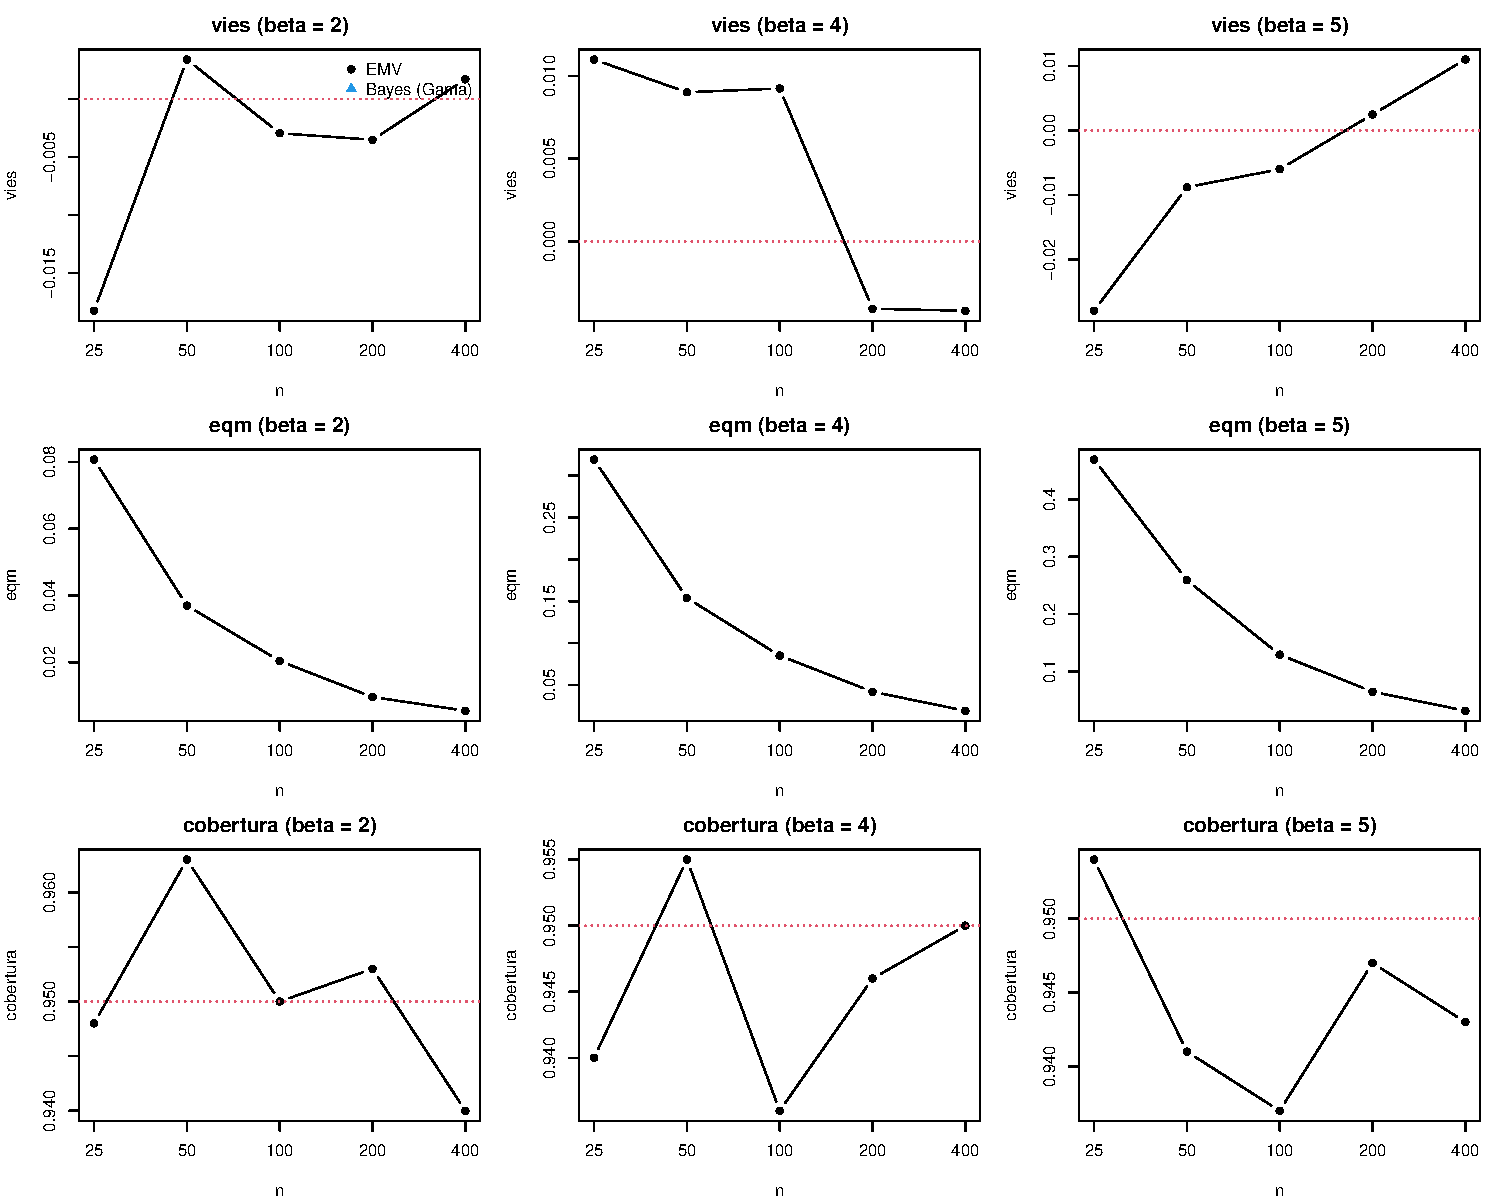
\includegraphics[width=\linewidth]{sim_comparacao.pdf}
\caption{Viés, EQM e cobertura em função de $n$ (escala log). Em preto, o EMV; em azul, a média a posteriori com a Priori 1. A linha vermelha marca o valor ideal.}\label{fig:simcomp}
\end{figure}

\begin{figure}[H]\centering
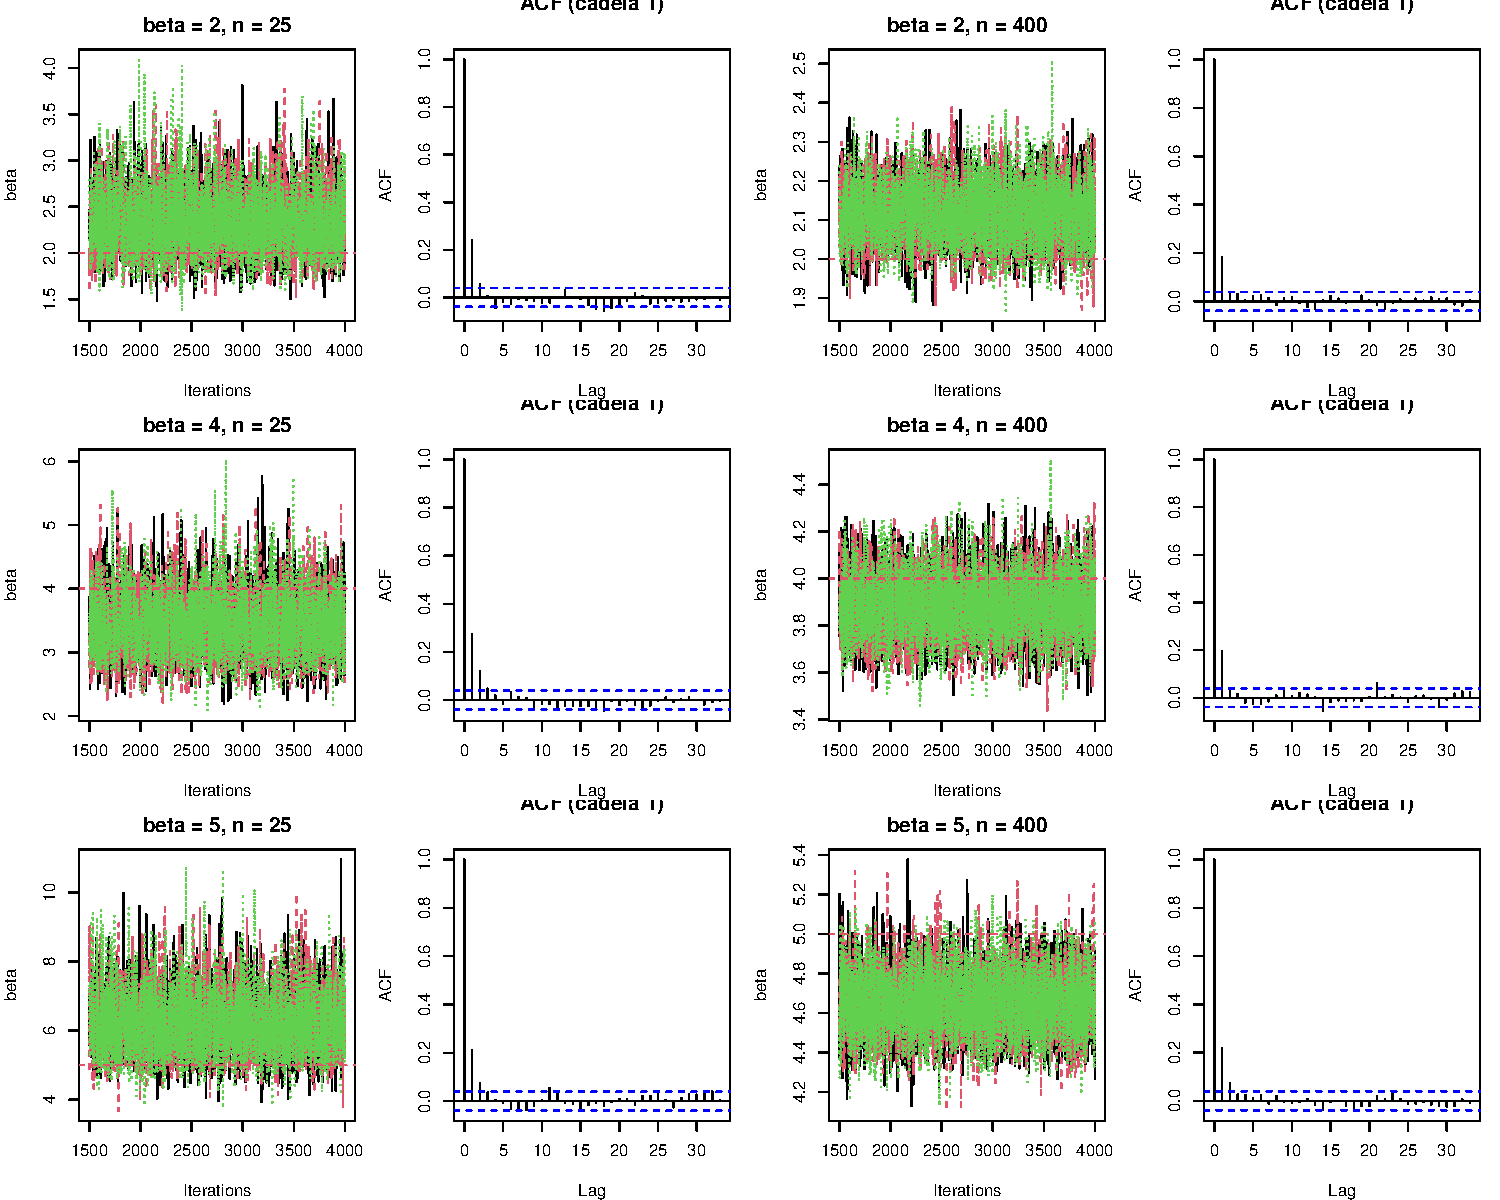
\includegraphics[width=\linewidth]{sim_convergencia.pdf}
\caption{Traço das 3 cadeias e ACF de uma réplica com $n=25$ e outra com $n=400$ para cada $\beta$. A linha tracejada marca o valor verdadeiro.}\label{fig:simconv}
\end{figure}

\paragraph{Discussão.} No caso clássico (Tabela~\ref{tab:simcl}), o EMV é praticamente não viesado em todos os cenários ($|\text{viés}|\le0{,}03$). O EQM decai como $1/n$: $n\cdot\text{EQM}$ fica perto de $2$, $8$ e $12{,}5$ para $\beta=2$, $4$ e $5$, ou seja, perto de $\beta^2/2$. Essa é a variância assintótica do EMV da escala de uma Gama de forma 2 contínua ($\Var\approx\beta^2/(2n)$), o que mostra que a discretização perde pouca informação sobre $\beta$. A cobertura do IC de Wald em $\log\beta$ fica entre 93,6\% e 96,3\%, próxima do nível nominal mesmo com $n=25$.

No caso bayesiano (Tabela~\ref{tab:simba} e Figura~\ref{fig:simcomp}), a média a posteriori tem um \textbf{viés positivo} em todos os cenários. Ele é pequeno e decai com $n$:
\begin{itemize}
\item com $n=25$, vale $+0{,}026$, $+0{,}098$ e $+0{,}078$ para $\beta=2$, $4$ e $5$;
\item com $n=400$, fica abaixo de $0{,}02$.
\end{itemize}
A causa é a assimetria da posteriori de um parâmetro de escala, não a priori: no intervalo $\beta\le5$, a densidade $\beta^{-0{,}9}e^{-0{,}01\beta}$ é praticamente $1/\beta$. Pela aproximação contínua, sob $1/\beta$ a posteriori de $\beta$ dado $\sum y_i$ é Gama inversa$(2n,\sum y_i)$. A média dela, $\sum y_i/(2n-1)$, supera a moda e o EMV, $\sum y_i/(2n)$, por um fator $2n/(2n-1)$. Isso dá um viés da ordem de $\beta/(2n)$, ou seja, $0{,}04$, $0{,}08$ e $0{,}10$ com $n=25$, compatível com o observado.

Mesmo assim, o EQM da média a posteriori é só 5--7\% maior que o do EMV com $n=25$ e fica igual (diferença $<1\%$) a partir de $n=200$. O intervalo de credibilidade é cerca de 2,5\% mais longo com $n=25$ e praticamente idêntico ao IC de Wald para $n\ge100$. A cobertura fica entre 93,8\% e 96,1\%.

Com $S=1000$, o erro de Monte Carlo da cobertura é $\sqrt{0{,}95\cdot0{,}05/1000}\approx0{,}7$ pontos percentuais. Assim, todas as coberturas, clássicas e bayesianas, são compatíveis com o nível nominal de 95\%.

Quanto à convergência (Tabela~\ref{tab:simconv} e Figura~\ref{fig:simconv}), \textbf{todas} as 15\,000 réplicas tiveram $\hat R<1{,}01$: o máximo foi 1,009, e o $\hat R$ médio ficou em torno de 1,0006. O ESS médio ficou entre 4350 e 4900 das 7500 amostras, com mínimo de 3212. Os traços mostram as 3 cadeias bem misturadas desde o fim do aquecimento, e a autocorrelação é desprezível após o lag 2.

Em resumo, com estas prioris e tamanhos amostrais, os dois paradigmas têm desempenho frequentista praticamente equivalente. O EMV leva uma pequena vantagem em viés quando $n$ é pequeno.

% =====================================================================
\section{Aplicação a dados reais}

\subsection{Dados}

Usamos os dois conjuntos de Afify et al. \cite{afify2022}, ambos de mortes diárias por COVID-19:
\begin{itemize}
\item \textbf{China}, de 23/01 a 28/03/2020 (worldometers): $n=66$, média 49,59, desvio padrão 44,02, índice de dispersão 39,1, CV 0,89;
\item \textbf{Europa}, de 01/03 a 31/03/2020 (OMS): $n=31$, média 785,8, desvio padrão 927,7, índice de dispersão 1095, CV 1,18.
\end{itemize}
Os dois são fortemente sobredispersos. O artigo lista os valores da China em ordem crescente, exceto por um ``3'' logo após o ``13''. Mantivemos os dados como publicados. No entanto, trocando esse 3 por 13, reproduzimos exatamente o EMV do artigo ($\hat\beta=25{,}122$ e $\ell=-330{,}515$); com o valor publicado, obtemos $\hat\beta=25{,}046$. Isso sugere um erro de digitação na lista impressa.

\subsection{Abordagem clássica}

\begin{table}[H]\centering\small
\caption{EMV, erro padrão e IC de 95\% (Wald na escala irrestrita) da DMEx e dos concorrentes.}\label{tab:apcl}
\begin{tabular}{lll rrrr}\toprule
Região & Modelo & Parâmetro & Estimativa & EP & IC inf. & IC sup.\\\midrule
\linhas{tabelas/aplic_classica.tex}
\bottomrule\end{tabular}
\end{table}

\begin{figure}[H]\centering
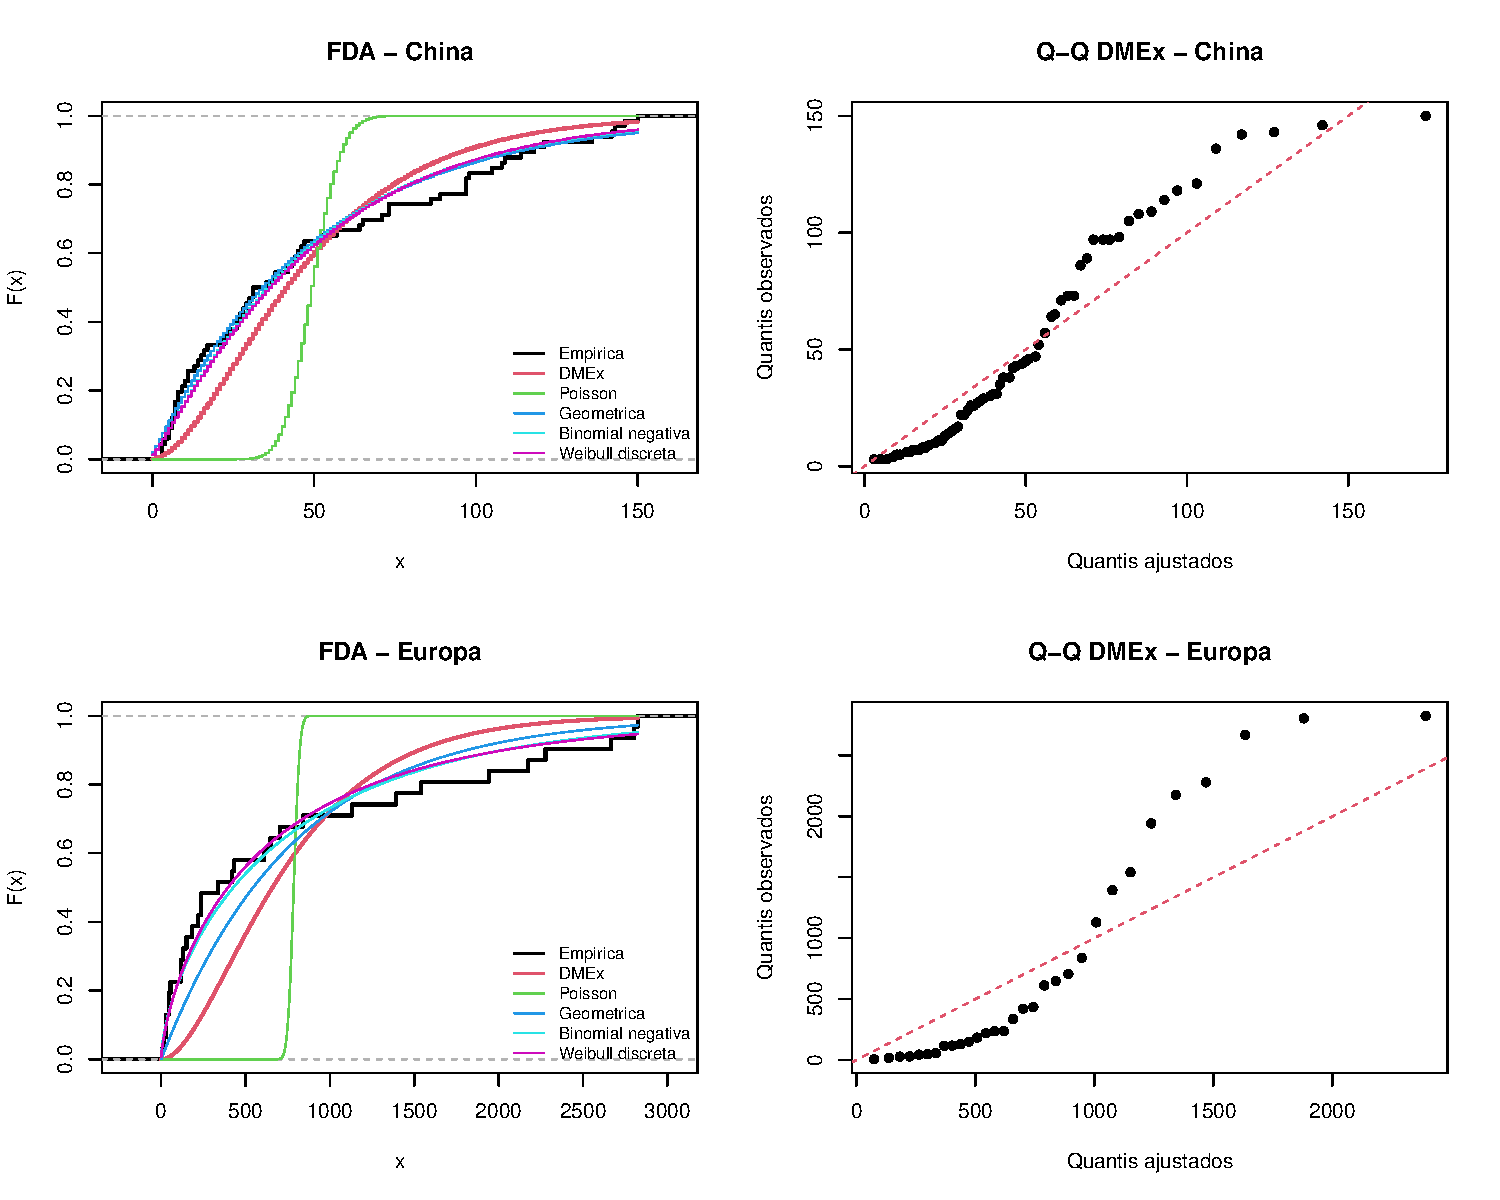
\includegraphics[width=0.95\linewidth]{ajuste_classico.pdf}
\caption{À esquerda, a FDA empírica e as FDAs ajustadas por máxima verossimilhança; à direita, o gráfico Q-Q discreto da DMEx.}\label{fig:apcl}
\end{figure}

\subsection{Abordagem bayesiana}

Ajustamos a DMEx com as duas prioris e os concorrentes com as prioris vagas de \texttt{comparacao\_bayes.R}:
\begin{itemize}
\item Poisson: $\lambda\sim\text{Gama}(0{,}1;0{,}01)$;
\item geométrica: $p\sim\text{Beta}(1,1)$;
\item binomial negativa: $\mu\sim\text{Gama}(0{,}1;0{,}01)$ e $r\sim\text{Gama}(2;0{,}1)$;
\item Weibull discreta: forma $\sim\text{Gama}(2,1)$ e escala $\sim\text{Gama}(0{,}1;0{,}01)$, também pelo ones trick.
\end{itemize}
Em todos, usamos 3 cadeias, adaptação 1000, aquecimento 5000 e 15000 iterações com desbaste 5, totalizando 9000 amostras.

\begin{table}[H]\centering\small
\caption{Resumo a posteriori: média, desvio padrão, intervalo de credibilidade de 95\% e $\hat R$. O ESS foi de pelo menos 8300 em todos os parâmetros.}\label{tab:apba}
\begin{tabular}{lll rrrrr}\toprule
Região & Modelo & Parâm. & Média & DP & 2,5\% & 97,5\% & $\hat R$\\\midrule
\linhas{tabelas/aplic_bayes.tex}
\bottomrule\end{tabular}
\end{table}

\begin{figure}[H]\centering
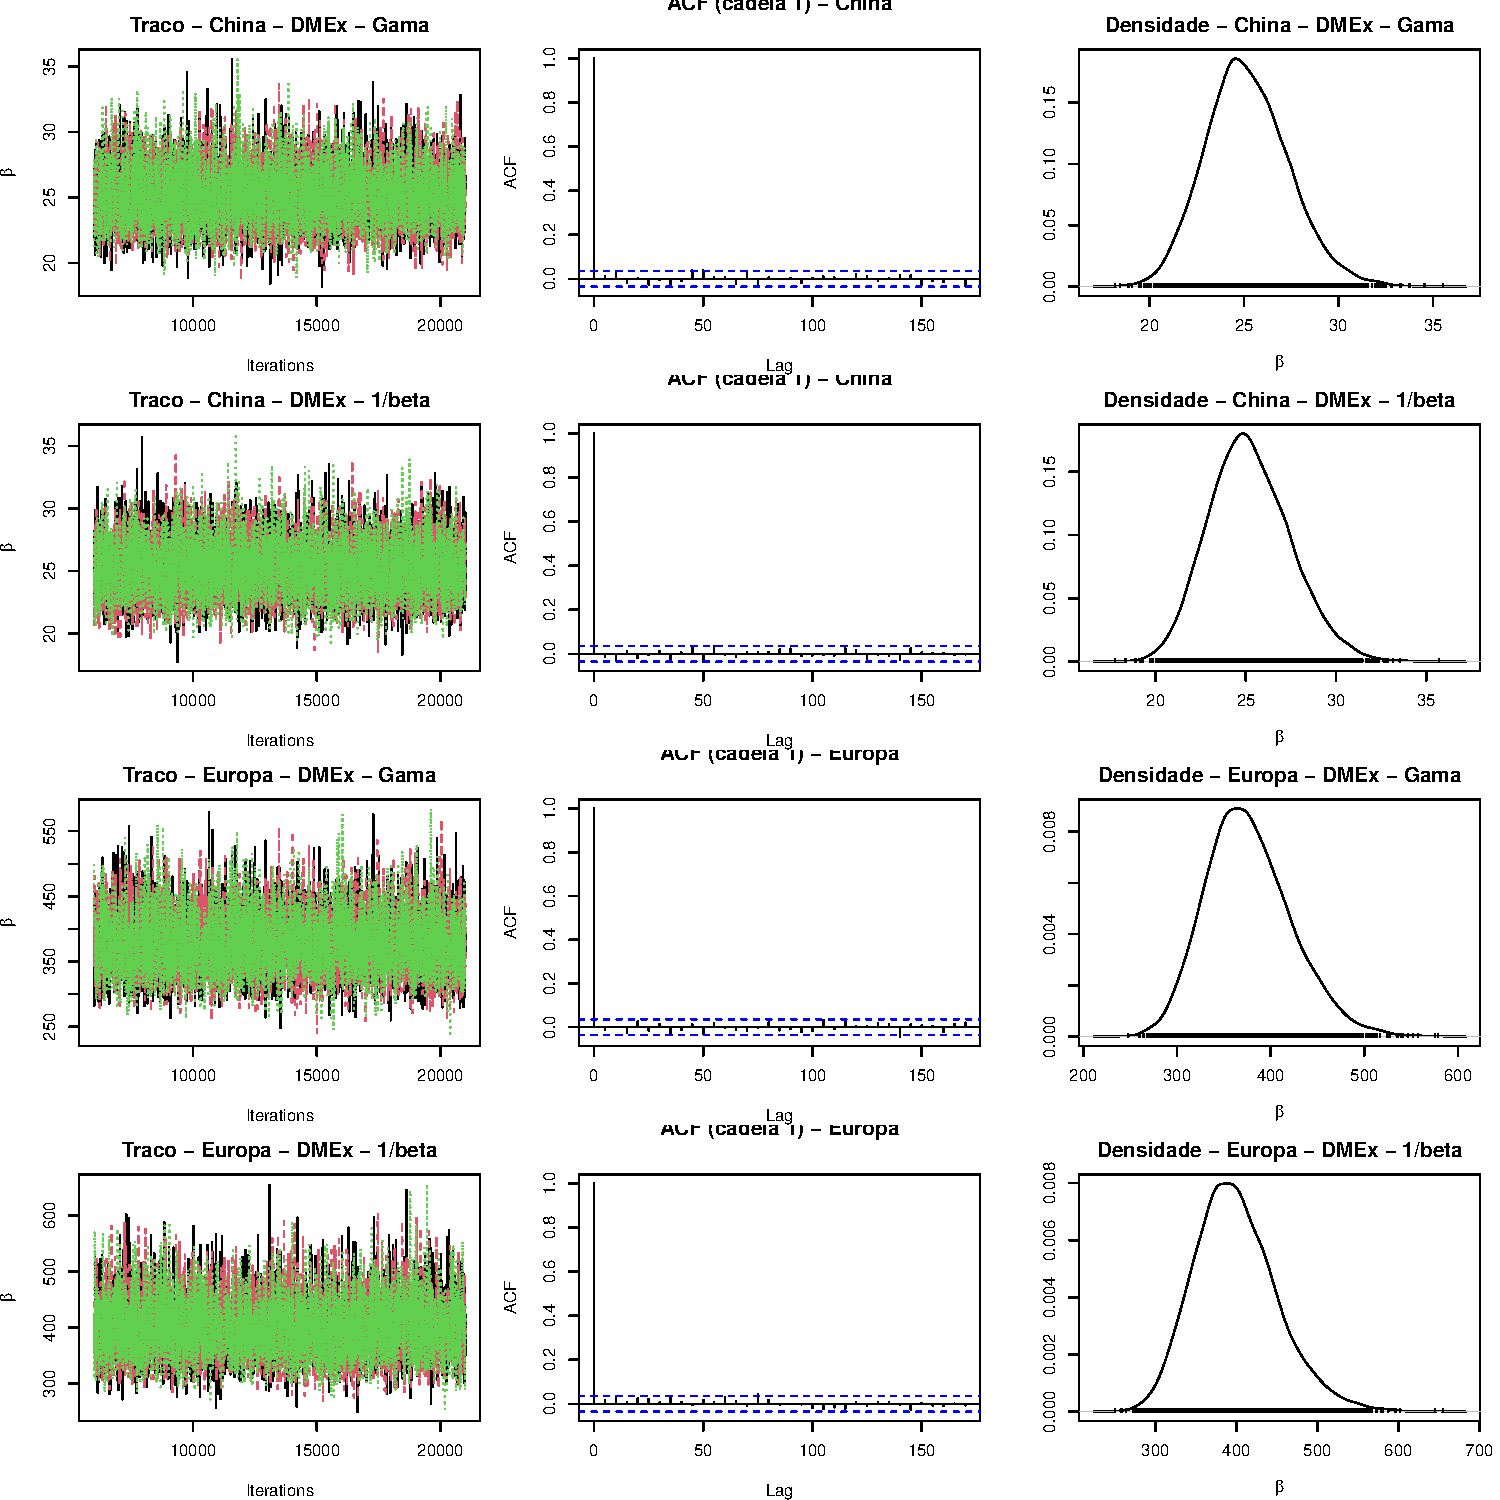
\includegraphics[width=0.95\linewidth]{diag_mcmc.pdf}
\caption{Diagnósticos da DMEx: traço das 3 cadeias, ACF e densidade a posteriori, por região e priori.}\label{fig:diag}
\end{figure}

\begin{figure}[H]\centering
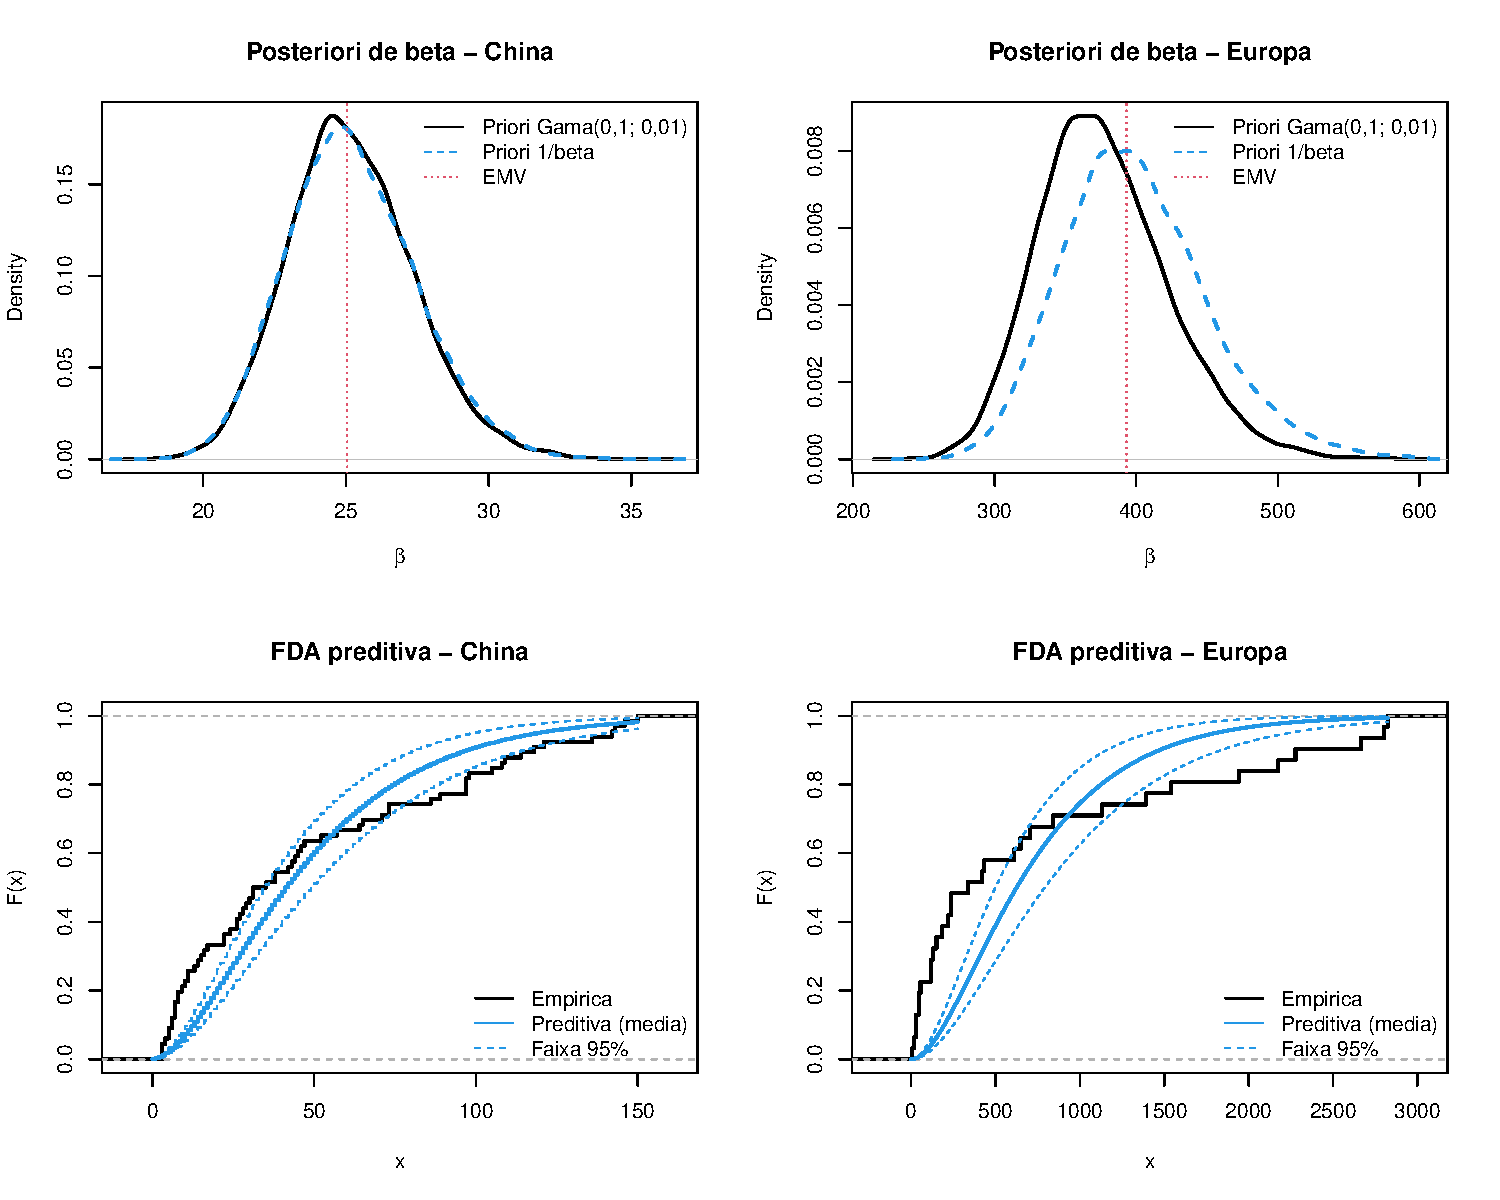
\includegraphics[width=0.95\linewidth]{bayes_aplicacao.pdf}
\caption{Acima, a posteriori de $\beta$ sob as duas prioris, com o EMV tracejado. Abaixo, a FDA preditiva a posteriori da DMEx com a Priori 1 (média e faixa pontual de 95\%) contra a FDA empírica.}\label{fig:apba}
\end{figure}

\begin{table}[H]\centering\small
\caption{Comparação de modelos: critérios clássicos (AIC, BIC) e bayesianos (DIC, WAIC, LPML). Os modelos estão ordenados pelo DIC dentro de cada região.}\label{tab:apfinal}
\begin{tabular}{ll rrrrr}\toprule
Região & Modelo & AIC & BIC & DIC & WAIC & LPML\\\midrule
\linhas{tabelas/aplic_final.tex}
\bottomrule\end{tabular}
\end{table}

\subsection{Discussão}

\paragraph{Estimação de $\beta$.} Na China, EMV ($25{,}05$; IC $[21{,}1;\,29{,}7]$) e posterioris (médias $25{,}20$ e $25{,}23$) praticamente coincidem, e as duas prioris dão a mesma posteriori (Figura~\ref{fig:apba}).

Na Europa a priori pesa mais. A média a posteriori é $376{,}8$ com a Gama$(0{,}1;\,0{,}01)$ e $399{,}6$ com $1/\beta$, contra o EMV de $393{,}2$. O motivo é o fator $e^{-0{,}01\beta}\approx e^{-4}$ da priori Gama em $\beta\approx400$: uma priori vaga na escala da simulação ($\beta\le5$) é informativa na escala destes dados. A priori $1/\beta$ é invariante por mudança de escala e não tem esse problema.

Todas as cadeias convergiram: $\hat R\le1{,}001$ e ESS $\ge8300$, com traços bem misturados e ACF desprezível após o desbaste.

\paragraph{Adequação e comparação.} A DMEx ajusta muito melhor que a Poisson, mas \emph{não} é o melhor modelo entre os considerados:
\begin{itemize}
\item na China, geométrica, Weibull discreta e binomial negativa têm AIC, DIC e WAIC cerca de 13 unidades menores e LPML maior;
\item na Europa, a diferença chega a cerca de 36 unidades.
\end{itemize}
O Q-Q e a FDA preditiva mostram a causa. A DMEx subestima a massa perto de zero e a cauda direita ao mesmo tempo, porque seu CV é fixo em $\approx0{,}71$, enquanto os dados têm CV de 0,89 e 1,18. A geométrica (CV $\approx1$) e os modelos de dois parâmetros acomodam melhor essa dispersão relativa.

O artigo original concluiu que a DMEx era a melhor porque a comparou com outro conjunto de concorrentes (Burr, Burr--Hatke, Rayleigh, Pareto, Topp--Leone inversa e Rayleigh inversa discretas, além da Poisson). Notamos também inconsistências na tabela do artigo para a Europa:
\begin{itemize}
\item o artigo dá $\hat\beta=409{,}36$ e $\ell=-257{,}12$;
\item nós obtemos $\hat\beta=393{,}17$ e $\ell=-255{,}76$, e o $\hat\beta$ do artigo dá $\ell=-255{,}81$ nos mesmos dados;
\item os AIC de vários concorrentes não conferem com $-2\ell+2k$.
\end{itemize}

% =====================================================================
\section{Considerações finais}

\begin{itemize}
\item \textbf{Modelo.} Deduzimos fmp, fda, taxa de falha, momentos, log-verossimilhança e escore analítico da DMEx, e verificamos tudo numericamente.
\item \textbf{Posteriori.} Mostramos que a posteriori sob $\pi(\beta)\propto1/\beta$, priori motivada pelo resultado de \cite{lindley1958}, é própria se, e somente se, a amostra tem alguma observação positiva.
\item \textbf{Simulação.}
  \begin{itemize}
  \item O EMV é praticamente não viesado, tem EQM próximo do limite assintótico $\beta^2/(2n)$ e cobertura próxima de 95\%.
  \item A média a posteriori tem um viés positivo da ordem de $\beta/(2n)$, que vem da assimetria da posteriori, e EQM até 7\% maior com $n=25$. As duas abordagens se equivalem a partir de $n\approx100$.
  \item O MCMC convergiu em todas as 15\,000 réplicas ($\hat R<1{,}01$ e ESS $\ge3200$).
  \end{itemize}
\item \textbf{Aplicação.} As inferências clássica e bayesiana concordam quando a priori é compatível com a escala dos dados. A priori Gama ``vaga'' mostrou-se informativa para $\beta$ na casa das centenas, o que recomenda a priori $1/\beta$ (invariante por escala) como padrão. Os critérios clássicos (AIC/BIC) e bayesianos (DIC, WAIC, LPML) concordam que a DMEx, por ter CV fixo, é superada pela geométrica, pela binomial negativa e pela Weibull discreta nos dados de COVID-19. Isso relativiza a conclusão do artigo original.
\end{itemize}

\paragraph{Propostas futuras.}
\begin{itemize}
\item Generalizar a DMEx com um parâmetro de forma, por exemplo a Gama discreta de forma $\alpha$, que tem CV livre.
\item Estudar a priori de Jeffreys exata do modelo discreto, que difere de $1/\beta$ para $\beta$ pequeno.
\item Incluir a priori $1/\beta$ e prioris Gama com hiperparâmetros na escala dos dados no estudo de simulação.
\item Tratar a dependência temporal das contagens diárias, que aqui foram supostas independentes, como no artigo original.
\end{itemize}

% =====================================================================
\appendix
\section{Códigos em R}

Os scripts estão em \texttt{R/} e devem ser rodados a partir da raiz do projeto, nesta ordem. Todas as funções do modelo ficam em \texttt{modelo.R}, que os demais carregam com \texttt{source()}.

\subsection*{modelo.R}\lstinputlisting{../R/modelo.R}
\subsection*{00\_checagens.R}\lstinputlisting{../R/00_checagens.R}
\subsection*{01\_amostras.R}\lstinputlisting{../R/01_amostras.R}
\subsection*{02\_sim\_classica.R}\lstinputlisting{../R/02_sim_classica.R}
\subsection*{03\_sim\_bayes.R}\lstinputlisting{../R/03_sim_bayes.R}
\subsection*{04\_aplicacao.R}\lstinputlisting{../R/04_aplicacao.R}
\subsection*{05\_tabelas\_figuras.R}\lstinputlisting{../R/05_tabelas_figuras.R}

% =====================================================================
\begin{thebibliography}{99}
\bibitem{afify2022} Afify, A. Z.; Ahsan-ul-Haq, M.; Aljohani, H. M.; Alghamdi, A. S.; Babar, A.; Gómez, H. W. (2022). A new one-parameter discrete exponential distribution: properties, inference, and applications to COVID-19 data. \emph{Journal of King Saud University -- Science}, 34(6), 102199. doi:10.1016/j.jksus.2022.102199.
\bibitem{dara2012} Dara, S. T.; Ahmad, M. (2012). \emph{Recent Advances in Moment Distribution and their Hazard Rates}. Saarbrücken: Lap Lambert Academic Publishing.
\bibitem{lindley1958} Lindley, D. V. (1958). Fiducial distributions and Bayes' theorem. \emph{Journal of the Royal Statistical Society B}, 20(1), 102--107.
\bibitem{nakagawa1975} Nakagawa, T.; Osaki, S. (1975). The discrete Weibull distribution. \emph{IEEE Transactions on Reliability}, R-24(5), 300--301.
\bibitem{roy2004} Roy, D. (2004). Discrete Rayleigh distribution. \emph{IEEE Transactions on Reliability}, 53(2), 255--260.
\bibitem{gelman1992} Gelman, A.; Rubin, D. B. (1992). Inference from iterative simulation using multiple sequences. \emph{Statistical Science}, 7(4), 457--472.
\bibitem{spiegelhalter2002} Spiegelhalter, D. J.; Best, N. G.; Carlin, B. P.; van der Linde, A. (2002). Bayesian measures of model complexity and fit. \emph{Journal of the Royal Statistical Society B}, 64(4), 583--639.
\bibitem{watanabe2010} Watanabe, S. (2010). Asymptotic equivalence of Bayes cross validation and widely applicable information criterion in singular learning theory. \emph{Journal of Machine Learning Research}, 11, 3571--3594.
\bibitem{geisser1979} Geisser, S.; Eddy, W. F. (1979). A predictive approach to model selection. \emph{Journal of the American Statistical Association}, 74(365), 153--160.
\bibitem{jags} Plummer, M. (2003). JAGS: a program for analysis of Bayesian graphical models using Gibbs sampling. \emph{Proceedings of the 3rd International Workshop on Distributed Statistical Computing (DSC 2003)}, Viena.
\bibitem{coda} Plummer, M.; Best, N.; Cowles, K.; Vines, K. (2006). CODA: convergence diagnosis and output analysis for MCMC. \emph{R News}, 6(1), 7--11.
\bibitem{ehlers} Ehlers, R. S. \emph{Introdução à Inferência Bayesiana}. Notas de aula, ICMC-USP.
\bibitem{syversveen} Syversveen, A. R. (1998). Noninformative Bayesian priors: interpretation and problems with construction and applications. Preprint, NTNU.
\bibitem{rcore} R Core Team (2026). \emph{R: A Language and Environment for Statistical Computing}. R Foundation for Statistical Computing, Viena.
\end{thebibliography}

\end{document}
